\section{Overview}

\subsection{Motivation}
Plasmas, commonly called the fourth state of matter, consist of neutral atoms or
molecules with some fraction split into pairs of electrons and positive (or
negative) ions. Initially, a curiosity of the laboratory (e.g.\ demonstrations
by Victorian-era scientists), they have become a critical part of every day
life. The electrically charged nature of plasmas makes them a practical means by
which to convert electrical energy into electromagnetic, chemical, kinetic, or
even nuclear energy. From an applications perspective, they are indispensable in
lighting, semiconductor manufacturing, plastic processing, and space propulsion.
On a more broad scale, virtually all observable light in the universe is derived
from the plasma state \cite{NA2007}.

Three things are required to create a plasma: matter, an energy source, and a
means of transferring the energy to the matter (often gas). In man-made
applications, the energy source is typically electricity, and the simplest
transfer mechanism is via two electrodes placed on either side of the gas. The
application of a potential difference to these electrodes produces an electric
field as seen in figure~\ref{fig:avalanche}.
\begin{figure}
  \centering
  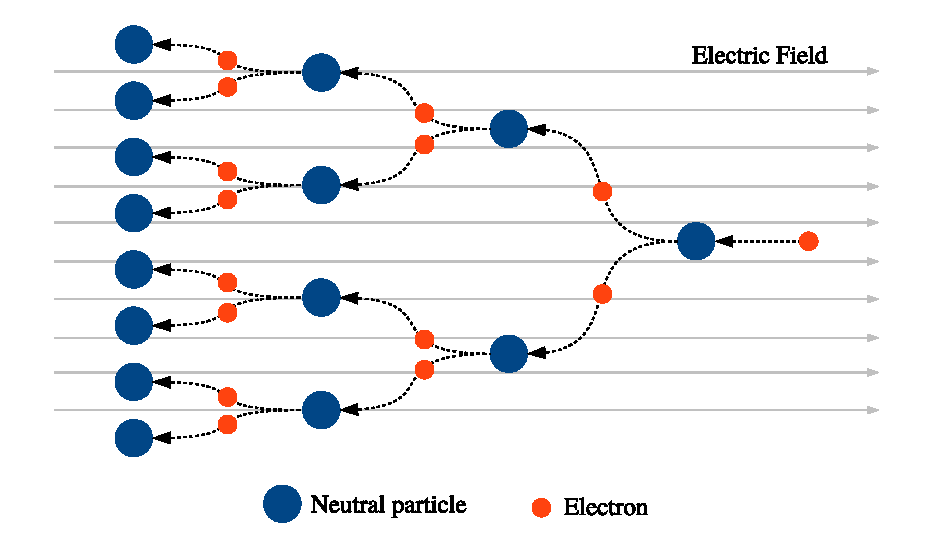
\includegraphics{./chapters/introduction/figures/avalanche.eps}
  \caption{A simplified depiction of the avalanche breakdown process in a gas.}
  \label{fig:avalanche}
\end{figure}
The field accelerates seed electrons in the gas (often created by background
cosmic radiation) until they collide with neutral particles. The seed electrons,
having acquired sufficient energy, liberate secondary electrons from the neutral
particles, leaving behind relatively heavy and immobile ions. Subsequently, both
the first and second electron are now accelerated by the electric field. Again,
they collide with two more neutral atoms, creating two new electrons. As long as
the electric field persists, the number of electron and ion pairs increases
exponentially. This process is generally referred to as an avalanche.

Eventually, the production of ions and electrons in the gap balances out with
the rate at which they leave the system, whether by collection at the electrodes
or by other processes (e.g.\ surface recombination or diffusion out of the
volume). The resulting ionized gas may be referred to as a plasma if it meets
certain criteria. Broadly speaking, these requirements can be expressed as,
\begin{enumerate}
  \item \textbf{Quasineutrality}: The density of the positive and negative
species are approximately the same.
  \item \textbf{Debye Shielding}: The system is large enough ($\lambda_\mathrm{D} 
<< L$) and possesses enough particles ($4\pi\lambda_\mathrm{D}^3/3 >> 1$) for
Debye shielding to occur \cite{Chen1984}. These terms will be defined in more
detail in Chapter~\ref{chp:theory}.
  \item \textbf{Electrostatic Effects}: The interaction of the charged particles
must dominate over the influence of random collisions with neutral gas particles
($\omega_\mathrm{p} > \nu$) \cite{Chen1984}.
\end{enumerate}

Despite this relatively simple recipe, the physical characteristics can vary
greatly depending on the type of gas, its pressure, the nature of the applied
voltage, the composition of the electrodes, etc. As a result, man-made plasmas
are generally produced under very specific conditions. For example, a plasma
etcher used in semiconductor manufacturing may need to operate operate at
pressures that are one ten-thousandth of atmospheric pressure with ultra-pure
(99.999\%) gases \cite{Greenberg1993a}.

Plasmas such as those produced in plasma etchers, feature ions and neutral gas
particles with temperatures that are below 1,000 K. Though this temperature is
relatively high compared to room temperature, it is well below the temperature
of the electrons which are typically in excess of 20,000 K. Plasmas which
exhibit this disparity in temperatures are often called nonequilibrium or
``low-temperature'' plasmas.

Conversely, there exists another class of plasmas where the electrons, ions, and
neutral particles can all be described by the same equilibrium temperature.
These are called equilibrium plasmas. As the pressure is increased, plasmas
become susceptible to what is known as the ionization instability. Depending on
the conditions, this can lead to a glow-to-arc transition which causes an
initially non-equilibrium plasma to become an equilibrium plasma
\cite{Kunhardt2000}. The resulting arcs can be used in application which include
cutting, welding, high-intensity lighting, and surface coating.

There are, however, a number of applications which would benefit from operation
at higher pressures with the attendant removal of complex and costly vacuum
systems, but with low-temperature ions and neutrals so as to avoid heat damage.
This has spurred a substantial amount of research on nonequilibrium
atmospheric-pressure plasmas (\acs{app}s) in recent years \cite{Becker2005,
Starikovskii2009, Nishihara2011, Laroussi2005, Walsh2006, Lu2006}. Ideally, such
a plasma could be generated at or near atmospheric pressure with hot electrons,
but minimal heating of surrounding gas. Born in the 1960's, this field of has
produced a variety of new types of discharges and capabilities. One of the more
ubiquitous examples is use of plasmas to process the surface of plastics so that
ink can adhere.

As mentioned, these applications promise to be the first of many for such
plasmas. More recently, there have been innovative proposals to use these
plasmas in water purification \cite{Malik2001}, wound sterilization
\cite{Ayan2009}, improved combustion engines \cite{Nishihara2007}, nanoparticle
production \cite{Ostrikov2011}, and more. However, each situation has its own
challenges when it comes to the design and development of a plasma source,
particularly at these elevated pressures. Particularly problematic is the
ionization instability which can lead \acs{app}s to the glow-to-arc transition.

There exist a few ways of getting around these instabilities. One example is the
dielectric-barrier discharge which passively regulates the amount of power which
can be deposited into the plasma \cite{Kogelschatz2003} by limiting charge flow.
Another example includes split-ring resonators which use natural feedback
mechanisms to damp out potential instabilities \cite{Iza2005}. The technique
considered here, referred to as the repetitively-pulsed nanosecond discharge, or
\acs{rpnd}, uses high voltage pulses which are so short that the instability
does not have time to develop \cite{Adamovich2008}. The \acs{rpnd} is a
nonequilibrium plasma which can operate at pressures ranging from approximately
$10^{-3}$--$1$ atmospheres \cite{Vasilyak1994}. At atmospheric pressure the
\acs{rpnd} can produce a uniform plasma in volumes on the order of 10 mL
\cite{Walsh2006}. As the pressure is reduced, the plasma volume can reach the
order of liters \cite{Starikovskaia1998}.

The importance of large-area, uniform, high-pressure plasmas such as the
\acs{rpnd} was highlighted in the National Academies' most recent decadal survey
of plasma science \cite{NA2007}. However, there is still much that is not known
about such plasmas. From the same survey, it is said that ``the full promise of
\acs{app}s will be known only if they can be understood and managed based on
fundamental scientific principles at two extremes--the nanoscopic kinetic level,
where selective chemistry occurs, and the global stability level.'' It is this
challenge, specifically the investigation of the nanoscopic kinetic level, which
drives the research presented here.

\subsection{History}

Historically, the study of low-temperature \acs{app}s has been almost
indistinguishable from the study of plasmas as a whole. However, this was not
necessarily a matter of reasoned choice. Plasma generation at
atmospheric-pressure obviates the need for a vacuum pump. Additionally, prior to
the creation of large battery banks, early sources of electrical energy had
relatively small capacities. This precluded the generation of thermal
atmospheric plasmas which required large amounts of energy.

The first spark discharge is commonly attributed to Thales of Mil\^{e}tus from
around 600 B.C. Following Thales, electrical sparks came to intrigue many
scientists including Gottfried Liebniz, Benjamin Franklin, and Charles
Wheatstone. By the mid-1800s, Pl\"{u}cker, Gei\ss{}ler, and Hittorf began some
of the first work on low-pressure plasmas though it was Crookes who would later
identify plasma as a separate state of matter. Later, J.J.\ Thomson's discovery
of the electron and discretized charge in 1897 marked the beginning of modern
plasma research.

By this time, the necessary tools and techniques existed to create steady
plasmas in rarified gases. These discharge tubes were ideal for basic studies of
plasma behavior and were used to great effect by individuals such as Lewi Tonks
and Irving Langmuir \cite{Tonks1929}. In fact, many modern concepts in plasma
physics can be traced back to their work.

In contrast, the pulsed \acs{app}s, characteristic of the earliest man-made
plasmas \cite{Anders2003}, were straightforward to create, but difficult to
carry out measurements upon. For many years, there were simply no instruments
with the necessary time resolution. Furthermore, neutral particles were present
in such quantities that they could confound or obscure otherwise simple
measurements.

Diagnostic capabilities and theory evolved to allow increasingly detailed
measurements on high pressure plasmas. This included lightning research which
utilized a number of novel photographic techniques beginning in the 1920's and
oscillographs and photographs of streamers starting in the 1930's. After World
War 2, photomultiplier tubes were introduced in the study of high pressure
discharges follow by fast digital imaging. 

Despite these advances, there is still a great deal that is not known about
about pulsed \acs{app}s, particularly lightning, streamers, and a type of plasma
which Thomson referred to as a ``luminous front.'' By the 1970s, this latter
plasma had come to be called the fast ionization wave, or \acs{fiw}
\cite{Vasilyak1994}. It was generated by a single voltage pulse lasting around
100 nanoseconds and peaking at 10s or 100s of kilovolts. For the right pressure
and gas, the \acs{fiw} could fill volumes of nearly 40 L with a relatively
uniform plasma, but with little heating of the gas.

An early example of applications for these discharges was in high-pressure
lasers. Specifically, copper \cite{Kushner1983} and copper halide
\cite{Pack1977} lasers drew a significant amount of attention. Similarly,
excimer lasers were also of substantial interest \cite{Shimada1985}. The
switching circuitry for these lasers generally involved either pressurized spark
gaps or thyratrons.

These switching mechanisms were somewhat limiting for the application of
\acs{fiw}s. Spark gaps possess a relatively long recovery time which limits
their repetition rate \cite{Moran1991}. As the lifetime of a plasma at elevated
pressures is relatively short this results in a relatively low plasma duty
cycle; the ratio of the time the plasma spends on to the time it spends off.
Thyratrons, did not have such limitations, however their high cost and low
lifetimes motivated a search for replacements \cite{Partlo1995}.

Fast-switching semiconductor devices (e.g.\ the thyristor and silicon-controlled
rectifier) eventually mitigated these limitations. At present, switches exist
which can reliably operate at 100 kHz; sufficiently fast that the
plasma duty cycle approaches 100\% \cite{Efanov1997}. The discharge produced by
the use of these new switches is what we refer to as the \acs{rpnd}.

\subsection{Questions}

A survey of pulsed plasma research shows that \acs{rpnd}s are still not
well-understood. One specific impediment to \acs{rpnd}s research has been the
time-scale related to their formation (on the order of nanoseconds). This small
time-scale results in very brief signals with low, time-integrated intensities.
Such signals necessitate sensitive detectors and diagnostic equipment
Unfortunately, such devices are often susceptible to the broadband electronic
noise generated by the current pulses in the \acs{rpnd}. Other \acs{rpnd}
properties such as the high collisionality relative to other plasmas and the
large electric fields have also hindered experimental measurements.

Consequently, the majority of \acs{rpnd} studies focus on measurements before
and after the discharge has occurred. The literature includes a moderate degree
of information is available for this period of time in particular \acs{rpnd}s.
Such data include chemical compositions, atomic densities, electron densities,
gas temperatures, and more, with an emphasis on molecular gases. Such
measurements can provide important insight on the conditions which preclude the
pulses of an \acs{rpnd} as well as the end results of the pulse, however they
only allow inferences of what occurs during the onset of the pulse.

Of particular importance is the flow of energy through the charged and neutral
states of the discharge. Initially, electrical energy flows into the seed
electrons, heating them and leading to ionization and excitation of the neutral
atoms and/or molecules. The rate at which electron-induced reactions occur is
primarily related to the distribution of kinetic energy amongst the electrons,
or the electron energy distribution function (\acs{eedf}). The \acs{eedf} plays
a large role in determining the composition of the plasma and how it evolves
over time. However, little effort has been made to investigate the effect of
\acs{eedf} assumptions on the predictive capabilities of \acs{rpnd} simulations.
Because of the fundamental role which the \acs{eedf} plays in discharge
properties, this indicates an important and unexplored avenue of research.

As previously mentioned, the \acs{eedf} determines the rate of electron-induced
reactions within the discharge. Such reactions produce many of the ions and
excited states which are typically the desired discharge products. These
particles are responsible for the light emissions, many of the chemical
reactions, and all of the material deposition which result from a discharge.
Again, only a moderate amount of work has attempted a detailed comparison of
simulated and experimental excited state dynamics. To some extent, this may be
attributed to a lack of accurate cross sections or rate coefficients, along with
the uncertainty related to the \acs{eedf}. In general, comparisons between
experimental and numerical predictions offers the opportunity to identify new
physics in the \acs{rpnd}. Similarly, such a comparison may yield additional
insight on the nature of the \acs{eedf}. Thus, a comparison of the experimental
and numerical excited state dynamics is a promising means to identify new
phenomena in the \acs{rpnd} and is complementary to an analysis of its
\acs{eedf} properties.

\subsection{Approach}

The dissertation presented here represents efforts to either answer or provide a
foundation to answer the aforementioned questions. In order to develop the
appropriate context for this work, the next section gives a comprehensive review
of the \acs{rpnd} literature. It begins with the first reported pulsed
\acs{app}s and concludes with contemporary studies.

The following two chapters establish the basis for the experimental and
numerical studies. Chapter~\ref{chp:theory} presents the theory necessary to
understand \acs{rpnd}s including streamer discharges, atomic spectroscopy, and
collision processes. Subsequently, Chapter~\ref{chp:experiment} describes the
design of the helium \acs{rpnd} discharge apparatus used for the experimental
studies and as the basis for the simulations. Also included in this chapter are
several measurements of the basic discharge properties.

Chapters~\ref{chp:metastables} through~\ref{chp:modeling} provide more detailed
measurements and analysis of the \acs{rpnd} dynamics. In
Chapter~\ref{chp:metastables}, the measurements of the helium metastables in a
\acs{rpnd} are presented and analyzed as a function of pressure an axial
location in the discharge apparatus. Chapter~\ref{chp:emissions} presents and
analyzes similar measurements of the spontaneous plasma emissions. Finally,
Chapter~\ref{chp:modeling} discusses the development of a global model for a
helium plasma and its use with the experimental data to infer the plasma
properties of the \acs{rpnd}. The dissertation concludes with a summary of the
results and suggestions for further avenues of research.

\section{Literature Review}

The study of \acs{rpnd}s originated in the study of \acs{fiw}s and the
subsequent work on high-pressure laser systems. The physics of their formation
is related to a more broad category of plasmas which includes lightning,
streamers, and even some transient phenomena in DC glows \cite{Loeb1965}. These
plasmas are unique in that their spatial structure develops at speeds much
faster than can be accounted for by the conventional Townsend mechanism. Loeb
refers to this phenomena as ``ionizing waves of potential
gradient.''\footnote{It should be noted that the phrase wave does not indicate
any kind of periodic motion or spatial arrangement. Simply put, it describes a
boundary which separates ionized and unionized gas which travels from one
electrode to another.}.

\subsection{Early History of Pulsed Discharges}

In 1835 (as reported by Thomson \cite{Thomson1893}), Charles Wheatstone
attempted to measure what he thought to be the speed of electricity in a
six-foot long discharge tube of unspecified pressure \cite{Wheatstone1835}. It
is now known that he was actually measuring the speed with which a plasma formed
between the two electrodes. He accomplished this by the use of a rotating mirror
which allowed him to see images of two sections of the tube, slightly displaced.
The displacement between the images was proportional to the speed with which the
plasma traveled between them. Wheatstone estimated this speed to be at least
$8\times10^7$ cm/s.

Interestingly, von Zahn later noted that this was \emph{not} the speed of the
emitting particles \cite{Zahn1879}. The visible light did cross the gap at an
appreciable speed, but there was no detectable Doppler shift in the light
emitted parallel to the propagation. As a result, it was concluded the
light-emitting particles could not be traveling at the same speed as the light.

Later, Thomson revisited this work with an improved apparatus
\cite{Thomson1893}. This included a tube that was now 15 m in length and five mm
in diameter, as seen in figure~\ref{fig:thomson}.
\begin{figure}
  \centering
  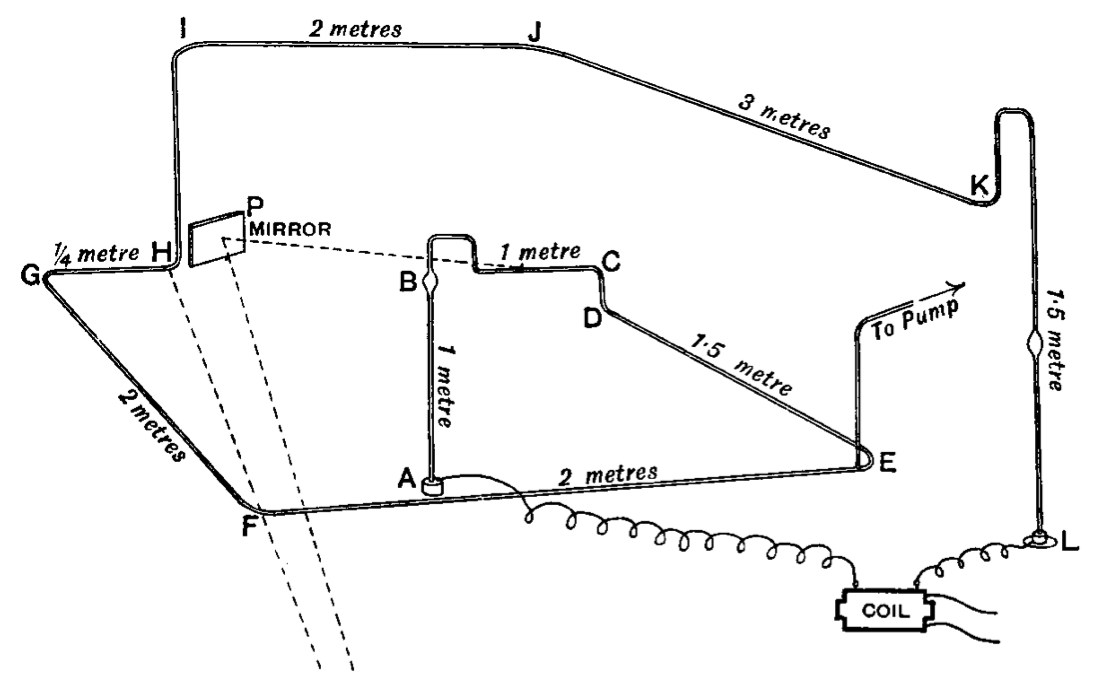
\includegraphics[width=4in]{chapters/introduction/figures/thomson.png}
  \caption{A sketch of J.J. Thomson's early experiments on pulsed plasmas 
  in long vacuum tubes \cite{Thomson1893}.}\label{fig:thomson}
\end{figure}
Also using the rotating mirror apparatus, Thomson was able to greatly improve on
the estimates of Wheatstone. He estimated that the so-called ``luminous front''
had a speed that was more than $1.5\times10^{10}$ cm/s, or in excess of half of
the speed of light. Furthermore, Thomson determined that the luminous front
always appeared to travel from the positively pulsed electrode (anode) to the
ground electrode (cathode).

The study of these luminous fronts was revisited by several researchers in the
wake of Thomson \cite{James1904, Whiddington1925, Beams1926}, but their attempts
to duplicate the measured speeds were met with varied success. In 1930, Beams
confirmed definitively confirmed those of Thomson. He also found that the front
always initiated at the electrode with the highest, absolute potential, relative
to ground. Beams hypothesized that the rapid motion of the front was a result of
a self-propagating region of high space charge, quote:
\begin{quote}
  In the neighborhood of the electrode $\ldots$ the field is very high and
  intense ionization should take place. This ionization due to the large
  difference in mobilities of positive ions, negative ions and electrons
  respectively should result in the establishment of a space charge. This space
  charge, once formed near the high potential electrode $\ldots$ must move
  down the tube regardless of the polarity of the applied potential because of
  the changes it produces in the field near its edges.
\end{quote}

At about the same time, Schonland and Collens reported on their observations of
lightning \cite{Schonland1933}. Though the general structure and length scale of
lightning is substantially different from the luminous fronts observed by Beams
and Thomson, the two phenomena would later prove to be very similar. In their
work Schonland and Collens noted that lightning would usually occur in a
two-step process. Based on the images they obtained, they suggested that
the leader was generated by a relatively small ``dart'' with a mean vertical
velocity of $7.2\times10^8$ cm/s. The dart moved in a random manner, changing
directions at random intervals, but always moving toward the ground.

The second step began when this dart reached the ground. Once there, a bright
return stroke would occur along the same path that the leader had traced out. In
contrast to the leader stroke, the return stroke had a velocity of $5\times10^9$
cm/s. Schonland and Collens hesitantly attributed the leader stroke to an
extended electron avalanche, and the return stroke to thermal ionization along
the conductive path generated by the dart. However, calculations by Cravath and
Loeb showed that the speeds of the proposed avalanche was inconsistent with the
fields at the head of a lightning stroke \cite{Cravath1935}. Instead, they
suggested that the dart was actually a moving region of space charge which
locally accelerated electrons to ionizing energies. This was similar to the
mechanism earlier proposed by Beams.

\subsection{The Streamer Model}

It was long known that sparks in air were similar to lightning. Advances in
technology during the 1930's led to experiments which reinforced this
similarity. In response to the measurements of Schonland and Collens; Snoddy,
Beams, and Dietrich studied the breakdown of gas in a long tube with both
positive and negative applied potentials \cite{Snoddy1936}. Using an
oscillograph, they observed both the leader and a return stroke in both cases.
However, the propagation of the plasma wave toward the cathode required a source
electrons ahead of the wave. The authors proposed that photoionization might
provide these necessary electrons.

Around the same time, Flegler and Raether had come to a similar conclusion
regarding the importance of photoionization. This led them to develop a more
thorough theoretical model for these waves \cite{Flegler1936} which came to be
known as the streamer theory. This was followed by a similar treatment by Loeb
and Meek \cite{Loeb1940, Loeb1940a, Meek1940}. The streamer theory divided the
initial plasma formation into two steps. In the first step, an electron
avalanche is initiated between two electrodes. The avalanche travels toward the
anode and leaves behind a region of positive space charge. In the second step,
the return stroke begins at the anode and travels along the conductive path
generated by the initial avalanche toward the cathode.

The streamer model proved relatively successful in describing the development of
sparks and lightning. Theoretical estimates of the speed matched the velocity
measurements that were acquired with photographs and oscillographs.
Additionally, the theory was able to account for the branching manner in which
lightning was formed as well as the constriction in space.

Following the initial work of Flegler, Raether, Loeb, and Meek, a number of
researchers began to explore the boundary between the Townsend mechanism and the
streamer mechanism. Most notable was Fisher and Bederson's work in 1951
\cite{Fisher1951}, which was later extended to nitrogen \cite{Kachickas1952} and
argon \cite{Kachickas1953}. These studies suggested that the streamer theory was
incomplete. Furthermore, the reliance of the streamer theory on photoionization
would later prove very contentious \cite{Kunhardt1988}. Finally, there was a
whole class of discharges that it did not readily explain.

\subsection{Diffuse Streamers}

As noted by Chalmers \cite{Chalmers1971}, Rogowski and Buss \cite{Rogowski1927,
Buss1932} observed a fast, diffuse, glow discharge immediately prior to the
filaments of a streamer discharge. Allibone and Meek, noted similar diffuse
discharges in air based on oscillographs and photographs \cite{Allibone1938,
Allibone1938b, Allibone1938c}. However, the Boys apparatus \cite{Boys1926} which
was employed in these studies (an ancestor to the modern streak camera) was
unable to capture the evolution of the diffuse glow, given its large spatial
extent.

This was first noted by Allibone who attempted to use Lichtenberg
figures\footnote{Such figures directly exposed photographic emulsions to the
electrical discharge. The developed image was a time-integrated representation
of the discharge.} to definitively capture this diffuse glow
\cite{Allibone1948}. Later, Saxe and Meek used the recently invented
photomultiplier tube to record the evolution of the light emissions in the
brief, diffuse glow \cite{Saxe1948} as a function of space. Both studies
agreed in the existence of the diffuse glow, despite some disagreement on the
nature of its geometry and propagation.

By 1968 (according to Kunhardt and Byszewski \cite{Kunhardt1980}), Stankevich
and Kalinin had provided the most firm evidence yet of a diffuse discharge in a
dense gas \cite{Stankevich1968}. This was later confirmed by experiments with a
pulsed nanosecond discharge by Mesyats, Bychkov, and Kremnev \cite{Mesyats1972}.
In their analysis, they concluded that photoionization could not play a role in
such short-lived discharges. The formation of their discharge only required
several nanoseconds, much shorter than the lifetimes of the excited states
responsible for photon emission. They suggested that the streamer model required
some extension.

In addition to the diffuse discharge, Stankevich and Kalinin also noted the
detection of x-rays with each pulse. This suggested the presence of high-energy
electrons impinging on the surface of the electrodes, despite the high
collisionality of the dense gas. Not only that, but the electron energies could
even exceed what would be expected from the vacuum electric fields
\cite{Babich1977}. The eventual conclusion was that the electric field
associated with the space charge at the head of the streamer produced very
energetic electrons which deposited their energy far from the streamer tip
\cite{Kunhardt1980, Babich1990}, allowing the streamer to spread out beyond the
diffusive region of the electrons.

It was based on the studies of the fast electrons in these discharges that
Mesyats, Bychov, and Kremnev proposed the use of a fast electron beam for
pumping high-pressure gas lasers. Similar work was conducted simultaneously by
Fenstermacher et al.~\cite{Fenstermacher1972}. Palmer \cite{Palmer1974}, and
Levatter and Lin \cite{Levatter1980} determined that there was a threshold
amount of preionization required to ensure homogeneity of the discharge. Hunter
\cite{Hunter1976}, and Koval'chuk and Mesyats \cite{Koval'chuk1976} later
proposed that such discharges be used for fast-closing switches. Gas lasers
\cite{Liu1973, Liberman1974, Pack1977, Kushner1983, Shimada1985} and fast
switches would drive much of the later research on fast, pulsed discharges.

Eventually the longitudinal version of these uniform discharges came to be known
as (\acs{fiw}s). A large body of Russian literature developed around their
study, though much of it has remained untranslated. In 1994, Vasilyak produced
an extensive review of these studies \cite{Vasilyak1994}. The data include wave
velocities for a variety of gases and pressures. Other parameters such as
attenuation coefficients for the waves, high energy electron currents, electric
field measurements, and a circuit model of the \acs{fiw} are also included.

\subsection{Repetitively-Pulsed Nanosecond Discharges}

The type of discharge originally studied by Babich, Loika, and Tarasova came to
be known as the fast ionization wave (\acs{fiw}). In the years following its
discovery, a substantial effort was made to document the properties of the
\acs{fiw} over a wide range of conditions. In these studies, the wave velocity,
current, and attenuation were the most frequently measured quantities. Much of
this work is summarized in a review by Vasilyak \cite{Vasilyak1994}. Also
reviewed are Slavin and Sopin's work which was the first to attempt a
computation of the \acs{eedf} in \acs{fiw}s \cite{Slavin1992}.

The experimental measurements and computational work reported by Vasilyak were
expanded on by a series of studies conducted at the Moscow Institute of Physics.
These are reviewed by Starikovskaia et al.~\cite{Starikovskaia2001} and included
measurements of the electron density, electric field, and energy coupling for
\acs{fiw}s in air, nitrogen, and hydrogen. The computational work by
Starikoskaia and Starikovskii \cite{Starikovskaia2001a} still represents the
most detailed study of the \acs{eedf} in nitrogen \acs{fiw}s.

However, Starikovskaia et al.\ noted that the usefulness of \acs{fiw}s were
limited, in part, by their repetition rates. The power supplies for \acs{fiw}s
were capacitor banks, charged in parallel, and discharged in series (also
referred to Marx banks). Unfortunately, the spark gaps used to trigger these
capacitor banks would not operate above a few hundred Hz. While previous work in
high-pressure lasers had used thyratrons to ameliorate this issue, the cost of
thyratrons limited their adoption. Eventually, the widespread availability of
cheap, reliable, fast, solid-state switches (e.g.\ silicon-controlled rectifiers
and thyristors) by the late 1980's provided an alternative approach to
repetitive breakdown. Later, the fast ionization dynistor made it was possible
to achieve repetition rates of 100 kHz \cite{Efanov1997}.

This led to a new class of repetitively-pulsed discharges, or the \acs{rpnd}.
These discharges operated at sufficiently high rates such that the electrons and
ions would persist in significant quantities between pulses. This meant that the
plasma duty cycle was increased by a significant amount. These improved
qualities of the \acs{rpnd} over the \acs{fiw} inspired a number of novel,
application-driven studies. This included:
\begin{itemize}
  \item Plasma-assisted combustion \cite{Pancheshnyi2006, Starikovskaia2006, 
        Adamovich2008}
  \item Magnetohydrodynamic energy bypass engines \cite{Macheret2002,
        Adamovich2008, Schneider2009a}
  \item Plasma actuators \cite{Starikovskii2009, Adamovich2009}
  \item High-pressure xenon lamps \cite{Nikandrov2008}
  \item Plasma medicine \cite{Ayan2009, Zimmermann2012}
  \item Water treatment \cite{Foster2013}
\end{itemize}
Though not specific to the \acs{rpnd}, Becker et al. \cite{Becker2005} provide
an extensive discussion of the potential uses for non-equilibrium air plasmas.

As a result, contemporary researchers have produced a significant amount of
literature on the operation of \acs{rpnd}s. More recently, there have been
detailed measurements of the gas temperatures \cite{Pilla2006, Pancheshnyi2006,
Nishihara2006, Bao2007, Lou2007, Pai2009, Zuzeek2010, Nishihara2011}, chemical
composition \cite{Bao2007, Lou2007, Pai2009}, electric fields \cite{Ito2009,
Ito2010, Muller2011a}, and energy coupling \cite{Macheret2006, Pancheshnyi2006}.
Notably, these studies have been generally restricted to molecular gases; air,
nitrogen, and occasionally, hydrogen.

Of particular interest is the work of Starikovskaia and Sarikovskii on the
numerical modeling of the \acs{eedf} in a nitrogen \asc{fiw}
\cite{Starikovskaia2001}. The study compares solutions of the two-term expansion
of the Boltzmann equation, a common approach to the approximation of
\acs{eedf}s, to the results produced by a zero-dimensional Monte Carlo model of
the discharge. Both steady-state and dynamic \acs{eedf} results were compared
and it was found that, in nitrogen, there was an excess of high energy electrons
in the dynamic \acs{eedf} produced by the Monte Carlo approach as compared to
the steady-state results. These results suggest that the use of equilibrium
solutions of the Boltzmann equation may not be appropriate in the analysis of an
\acs{rpnd}. It is unclear if such results also apply to rare gas systems which
possess a very different set of reaction pathways for electrons with
correspondingly different cross sections.

Also notable is the work of Urabe et al.\ in the measurement of helium metastable
density profiles in a atmospheric-pressure helium jet \cite{Urabe2010}. While
the pulse used to generate the jet and its pressure are different from the
results presented in this work, some of the underlying physics of formation,
such as the impact of space charge, and the technique used, absorption
spectroscopy, are similar. Most notable is the observation of an annular
distribution of helium metastable states during positive voltage pulses. This is
attributed to the large local electric fields near the walls of the discharge
tube which are responsible for the initiation of the discharge. While Urabe et
al.\ use the metastable measurements to analyze the non-monotonicity of the jet
discharge, they do not attempt to analyze the results in the context of a
numerical model.

Overall, there has been a decline in the study of \acs{fiw}s, and relatively
little on large-volume \acs{rpnd}s. One of the most recent \acs{fiw} studies was
produced by Takashima et al. \cite{Takashima2011}. In it, the authors reported
on \acs{fiw}s in helium and nitrogen which were studied using capacitive probes
and voltage-current characteristics. The results were compared to extensive
two-dimensional fluid simulations and an analytic, one-dimensional drift model.
In most cases, the measurements and simulations showed good agreement.

\section{Summary}

Contemporary \acs{rpnd} studies have mostly focused on measurements in the
afterglow plasma or of time-integrated quantities. Some exceptions to this
include the work by Anikin et al. \cite{Anikin1998} and Takashima et al.
\cite{Takashima2011} to measure the electric field in \acs{fiw}s with capacitive
probes. This has limited the understanding of how \acs{rpnd}s develop as only so
much can be inferred from these measurements. Particular issues, such as the
electron energetics in the wave front are not firmly known. Numerical estimates
are available for the electron temperatures, however measurements are associated
with a high uncertainty stemming from the associated distribution assumptions.
Relatedly, the relative importance of photoionization and nonlocal electrons is
still under debate. Each of these issues is important in the development of a
thorough theoretical understanding of \acs{rpnd}s, as well as the validation of
simulations, and optimization for real world applications.

Relatedly, the study of \acs{rpnd}s has generally been limited to molecular
gases such as air, nitrogen, oxygen, or combustion-related mixtures.
Consequently, little information has been published on rare gas \acs{rpnd}s, in
spite of the fact that their unique physics makes them ideal for certain uses.
For example, some rare gas discharges exhibit very little gas heating, making
them desirable for the treatment of highly sensitive materials. Additionally,
the radiative emissions of rare gases have a range of uses from commercial
lighting to gas lasers. Finally, the large degree of Penning ionization
resulting from rare gases may make them useful in \acs{rpnd} gas mixtures as a
means of optimizing discharge properties.

\section{Scope of Thesis}

In order to address these issues, this work will use a combination of
experiments and modeling to examine the plasma dynamics of a helium \acs{rpnd}
on time scales ranging from 5 ns to 100 $\mu$s and at pressures from 0.3 to 16.0
Torr. The nanosecond time scale results will be one of a very few datasets
available on the evolution of the \acs{rpnd} during its formation. The aim of
this work is to provide new insight on the dominant physical processes in the
wave front. To complement this, the microsecond time scale measurements will
be used to probe the dominant loss mechanisms in between pulses as well as the
time-averaged characteristics of the \acs{rpnd}. Lastly, the parameterization
with pressure will offer the opportunity to examine how the physics of the discharge
is altered by the collisionality.

Experimentally, the \acs{rpnd} is studied through the analysis of its current
and voltage characteristics, optical emission, and with laser absorption
spectroscopy. The current and voltage characteristics will be used to determine
the energy absorbed by the plasma with each pulse. The energy coupled into the
plasma provides a point of comparison with other discharges and a basis on which
to estimate the energy required to generate individual excited states and ions.

Subsequently, the optical emissions will provide information about the excited
state dynamics and the wave velocity. As with the coupled energy, the wave
velocity provides a point of comparison to previous work, particularly the
results compiled by Vasilyak et al. \cite{Vasilyak1994} related to the
properties of \acs{fiw}s. The optical emissions, while not absolute measurements
of the excited state densities, will illustrate the relative population of
various excited states and their dynamics during the onset of the pulse and in
the afterglow. Additionally, these measurements will clarify the progression of
energy from the accelerated electrons to the neutral particles.

Finally, the laser absorption spectroscopy will be used to resolve the short
time scale dynamics and as a benchmark for the numerical modeling. The modeling
will focus on the development of a detailed global model of a helium discharge.
This model will be supported by additional particle-in-cell simulations, and
solutions of the Boltzmann equation. Using the metastable measurements as a
baseline, the global model will be used to predict the electric field, electron
temperature, electron density, excited state densities, and emissions of the
\acs{rpnd}. These results can then be compared back to the optical emission
measurements in order to determine self-consistency, analyze the validity of
\acs{eedf} assumptions in the development of the global model, and to identify
important physical phenomena in the \acs{rpnd}.
